\documentclass[12pt]{article}

\title{ET4340 Electronics for Quantum Computing\\Homework 5}
\author{
    Mick van Gelderen\\4091566
}
\date{December 2013}

\usepackage[utf8]{inputenc}
\usepackage[a4paper,margin=2.2cm]{geometry}
\usepackage{natbib}
\usepackage{graphicx}
\usepackage{listings}
\usepackage{framed}
\usepackage{mathtools}
\usepackage{braket}
\usepackage{ifmtarg}
\usepackage{multirow}
\usepackage{xfrac}
\usepackage{xcolor}
\usepackage{caption}
\usepackage{subcaption}

% Flat UI colors MUAHAHA

\definecolor{turquoise}{HTML}{1ABC9C}
\definecolor{emerland}{HTML}{2ECC71}
\definecolor{peter-river}{HTML}{3498DB}
\definecolor{amethyst}{HTML}{9B59B6}
\definecolor{wet-asphalt}{HTML}{34495E}
\definecolor{green-sea}{HTML}{16A085}
\definecolor{nephritis}{HTML}{27AE60}
\definecolor{belize-hole}{HTML}{2980B9}
\definecolor{wisteria}{HTML}{8E44AD}
\definecolor{midnight-blue}{HTML}{2C3E50}
\definecolor{sun-flower}{HTML}{F1C40F}
\definecolor{carrot}{HTML}{E67E22}
\definecolor{alizarin}{HTML}{E74C3C}
\definecolor{clouds}{HTML}{ECF0F1}
\definecolor{concrete}{HTML}{95A5A6}
\definecolor{orange}{HTML}{F39C12}
\definecolor{pumpkin}{HTML}{D35400}
\definecolor{pomegranate}{HTML}{C0392B}
\definecolor{silver}{HTML}{BDC3C7}
\definecolor{asbestos}{HTML}{7F8C8D}

\lstset{
        language=Matlab,                                % choose the language of the code
%       basicstyle=10pt,                                % the size of the fonts that are used for the code
        numbers=left,                                   % where to put the line-numbers
        numberstyle=\footnotesize,                      % the size of the fonts that are used for the line-numbers
        stepnumber=1,                                           % the step between two line-numbers. If it's 1 each line will be numbered
        numbersep=5pt,                                  % how far the line-numbers are from the code
        backgroundcolor=\color{clouds},          % choose the background color. You must add \usepackage{color}
        showspaces=false,                               % show spaces adding particular underscores
        showstringspaces=false,                         % underline spaces within strings
        showtabs=false,                                         % show tabs within strings adding particular underscores
%       frame=single,                                           % adds a frame around the code
        tabsize=2,                                              % sets default tabsize to 2 spaces
%       captionpos=b,                                           % sets the caption-position to bottom
        breaklines=true,                                        % sets automatic line breaking
        breakatwhitespace=false,                        % sets if automatic breaks should only happen at whitespace
        escapeinside={\%*}{*)}                          % if you want to add a comment within your code
}

\newcommand{\pauli}[1]{
    \ensuremath{
        \begin{bmatrix}
            \if#1x
                0 & 1 \\
                1 & 0 \\
            \fi\if#1y
                0 & -i \\
                i & 0 \\
            \fi\if#1z
                1 & 0 \\
                0 & -1 \\
            \fi
        \end{bmatrix}
    }
}

\setlength{\parindent}{0cm}

\newcommand{\paulisigma}[1]{%
    \ensuremath{\sigma{}_{#1}}%
}

\newcommand{\bmat}[1]{\begin{bmatrix}#1\end{bmatrix}}
\newcommand{\rsqrt}[1]{\ensuremath{\frac{1}{\sqrt{#1}}}}

\setlength{\parskip}{0.5em plus4mm minus3mm}
\newenvironment{answer}{\begingroup\setlength{\leftskip}{-\leftmargin}\begin{framed}}{\end{framed}\endgroup}

\newcommand{\CNOT}[1]{\ensuremath{\texttt{CNOT}_{#1}}}
\newcommand{\CPHASE}[1]{\ensuremath{\texttt{CPHASE}_{#1}}}
\newcommand{\SWAP}[1]{\ensuremath{\texttt{SWAP}_{#1}}}
\newcommand{\cnotgr}[1]{\ensuremath{\bmat{%
        1 & 0 & 0 & 0 \\%
        0 & 1 & 0 & 0 \\%
        0 & 0 & 0 & 1 \\%
        0 & 0 & 1 & 0 \\%
}}}

\newcommand{\degcel}[1]{\ensuremath{#1^{\circ}}}

\begin{document}

\maketitle

\paragraph{Problem 1: Warmup exercises} \hfill

\begin{enumerate}
    \item Consider an operator $M$ and one of its eigenstates $\ket{\psi}$ (with eigenvalue $\lambda$). Consider another operator $A$ that anticommutes with $M$ (i.e., $\{M,A\} \equiv MA + AM = 0$). Show that the state $A\ket{\psi}$ is an eigenstate of $M$ with eigenvalue $-\lambda$.

    \begin{answer}
        We can write $M\ket{\psi} = \lambda\ket{\psi}$.
        \begin{align*}
            MA + AM &= 0 \\
            MA\ket{\psi} + AM\ket{\psi} &= 0 \\
            MA\ket{\psi} + A\lambda\ket{\psi} &= 0 \\
            M\left(A\ket{\psi}\right) &= -\lambda\left(A\ket{\psi}\right)
        \end{align*}
    \end{answer}

    \item Now consider an operator $B$ that commutes with $M$ (i.e., $[M,B] \equiv MB - BM = 0$). Show that the state $B\ket{\psi}$ is an eigenstate of $M$ with eigenvalue $\lambda$.

    \begin{answer}
        Assuming M again has an eigenstate $\ket{\psi}$ with eigenvalue $\lambda$.
        \begin{align*}
            MB - BM &= 0 \\
            MB\ket{\psi} - BM\ket{\psi} &= 0 \\
            M\left(B\ket{\psi}\right) &= \lambda\left(B\ket{\psi}\right)
        \end{align*}
    \end{answer}

    \item Prove the identity:

    \begin{center}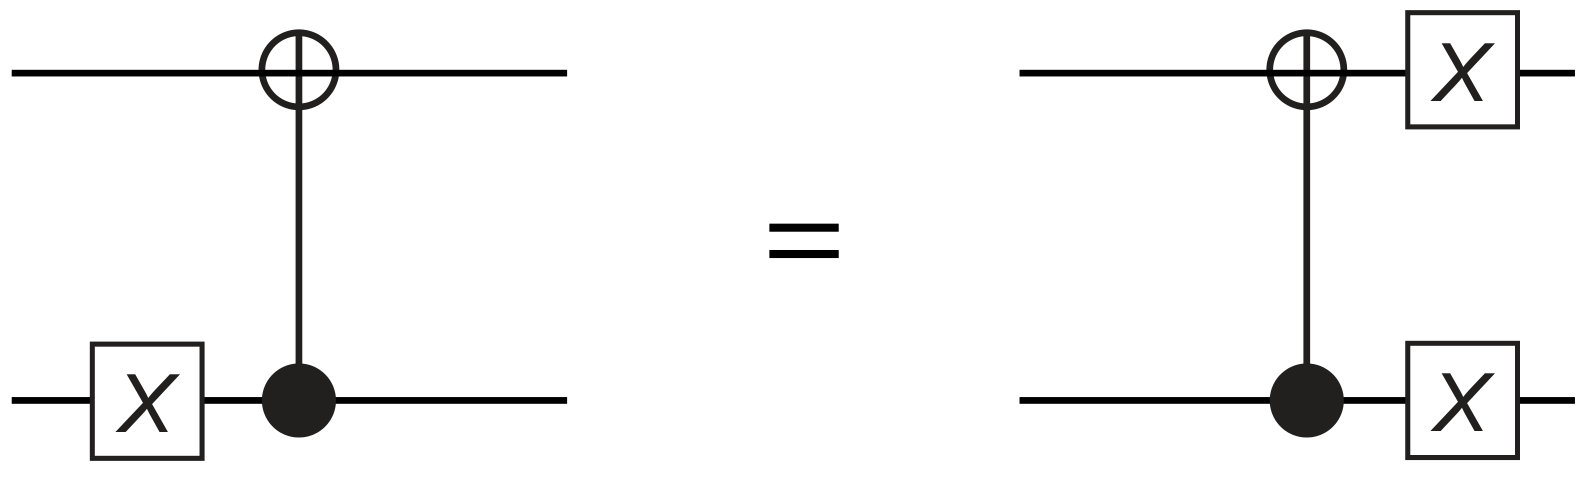
\includegraphics[width=.8\textwidth]{problem-1.png}\end{center}

    Feel free to do this either by multiplying matrices or by manipulating circuit diagrams. From this we see that a single-qubit bit-flip error prior to \CNOT{} proliferates into a double bit-flip error.

    \begin{answer}
        It is an intuitive identity in my opinion. Flipping the control bit flips the output. So to `simulate' the flip before a \CNOT{} you can flip both the output and the control after the \CNOT{}.

        By matrice multiplication (note that the order of operations is reversed with respect of the diagram because we compute the combined matrix $M = M_n\dots{}M_2M_1$ in $\ket{out} = M\ket{in}$ where $M_n$ is operation $n$):
        \begin{align*}
            M_a &= \CNOT{01}(I \otimes X) &=
                \bmat{1&0&0&0\\0&0&0&1\\0&0&1&0\\0&1&0&0}
                \bmat{0&1&0&0\\1&0&0&0\\0&0&0&1\\0&0&1&0} &=
                \bmat{0&1&0&0\\0&0&1&0\\0&0&0&1\\1&0&0&0}\\
            M_b &= (X \otimes X)\CNOT{01} &=
                \bmat{0&0&0&1\\0&0&1&0\\0&1&0&0\\1&0&0&0}
                \bmat{1&0&0&0\\0&0&0&1\\0&0&1&0\\0&1&0&0} &=
                \bmat{0&1&0&0\\0&0&1&0\\0&0&0&1\\1&0&0&0}\\
            M_a &= M_b
        \end{align*}
    \end{answer}
\end{enumerate}

\paragraph{Problem 2: Three-qubit bit flip code} \hfill

Consider the 3-qubit bit-flip code as covered in the lectures. In this code, a one-qubit state $\ket{\psi} = \alpha\ket{0_2} + \beta\ket{1_2}$ is encoded as $\ket{\Psi} = \alpha\ket{0_30_20_1} + \beta\ket{1_31_21_1}$.

\begin{enumerate}
	\item Suppose the encoded state is distorted by a rotation of $\degcel{60}$ about the $+\hat{x}$ axis of qubit 3. What are the possible error syndromes you could measure (i.e., the measurement results $m_a$ and $m_b$)? Show that the state $\ket{\Psi}$ is recovered after error correction, every time.

	\begin{answer}
		Since the distortion is not a full flip you can measure qubit 3 as either $-1$ or $+1$. The other two bits are not affected and will retain their (equal) states.

		The $Z$ (parity) measurement $m_a$ of qubits $q_1$ and $q_2$ will always give $m = +1$ because $q_1 = q_2$. The same does not hold for qubits $q_2$ and $q_1$, you will measure $m = \pm1$ by chance.

		The error syndromes thus are $m_a = +1, m_b = +1$ and $m_a = +1, m_b = -1$. In the first case you won't have to do anything. In the second case you will have to flip qubit $q_3$ back.

        Thus the final state is always `correct' or valid so to speak.
	\end{answer}

	\item Suppose now that instead the encoded state is distorted by a rotation of $\degcel{45}$ about the $+\hat{y}$ axis of qubit $q_2$, but you don't know it and stick to using the bit flip code without modifications. What are the possible error syndromes you would measure? Can you recover the state $\ket{\Psi}$ every time? When do you succeed and when do you not? When you don't recover it, what is the erroneous final state of the logical qubit?

	\begin{answer}
		This time we apply a maybe-$Y$ gate to qubit $q_2$. Since $Y = iXZ$ and the measurements we perform are two $Z$ measurement, we can make some conclusions about the different cases.

		We can recover the error when the $q_2$ becomes $Xq_2$ because the syndrome is $m_a = -1, m_b = -1$. This syndrome induces a flip on $q_2$ which makes $XXq_2 = q_2$.

        When $q_2$ becomes $Zq_2$, the syndrome is $m_a = +1, m_b = +1$. The final state in this case is $\ket{\Psi} = \alpha\ket{0_3+_21_1} + \beta\ket{0_3-_21_1}$.

        I think my answer is in the right direction but I'm having trouble writing it down and proving it mathmatically.
	\end{answer}
\end{enumerate}

\paragraph{Shor's 9-qubit code} \hfill

Consider Shor's 9-qubit code as covered in the lecture.

\begin{center}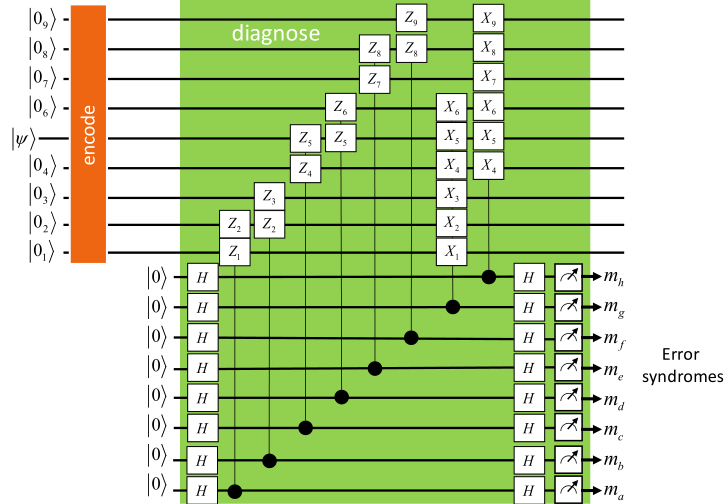
\includegraphics[width=1\textwidth]{problem-3.png}\end{center}

\begin{enumerate}
    \item Suppose a phase flip occurred on qubit $q_4$. What error syndromes ($m_a, \dots, m_h$) will you measure?

    \begin{answer}
        A phase flip means a $Z$ transition so the error syndrome for $Z_4$ is $m_g,$ $m_h$. I will write down only the abnormal measurements ($m = -1$).
    \end{answer}

    \item Now suppose a phase flip occured on qubit $q_5$.

    \begin{answer}
        The syndrome for $Z_5$ is $m_g$, $m_h$ as well.
    \end{answer}

    \item Now suppose a phase flip occured on qubit $q_6$.

    \begin{answer}
        The syndrome for $Z_6$ is $m_g$, $m_h$ as well.
    \end{answer}

    \item Explain the results from the previous three assignments.

    \begin{answer}
        Apparently we get the same syndrome when a phase flip occurs on qubits $q_4$, $q_5$ and $q_6$. Judging from Shor's previous work there has to be something clever going on behind the scenes here.

        The fact is that we can fix a phase flip on a qubit $q_z$ that is in any of the sets of three qubits $q_1 \cdots q_3$, $q_4 \cdots q_6$ and $q_7 \cdots q_9$ by performing a phase flip in any one (or all three) of the qubits in the set of qubits that $q_z$ is in. So $Z_4$ can be fixed by doing a $Z$ on qubit $q_4$, $q_5$ or $q_6$ (or all three).

        This property follows from the fact that if you do an even number of $Z$ transformations, the state of the logical cubit will stay the same.

        Lets see what $Z_2$ does:
        \begin{align*}
            (I \otimes Z \otimes I)\left(\alpha\ket{000} + \beta\ket{111}\right) =
                \bmat{
                    1&0&0&0&0&0&0&0\\
                    0&1&0&0&0&0&0&0\\
                    0&0&-1&0&0&0&0&0\\
                    0&0&0&-1&0&0&0&0\\
                    0&0&0&0&1&0&0&0\\
                    0&0&0&0&0&1&0&0\\
                    0&0&0&0&0&0&-1&0\\
                    0&0&0&0&0&0&0&-1\\
                }\bmat{\alpha\\0\\0\\0\\0\\0\\0\\\beta} = \bmat{\alpha\\0\\0\\0\\0\\0\\0\\-\beta}
        \end{align*}
        This just demonstrates that a $Z$ transformation indeed does not affect $\alpha\ket{000}$ and flips the phase of $\beta\ket{111}$.
    \end{answer}

    \item Suppose you measure the syndromes $m_a = m_b = m_c = m_d = m_g = m_h = -1, m_e = m_f = +1$. What error does this syndrome detect? Hint: it is not a single-qubit error. Interestingly, this shows that Shor's code can correct at least some two-qubit errors!

    \begin{answer}
        Table \ref{table:shor} table describes what cubits parity measurements are affected by which transformations ($X$, $Y$ or $Z$ errors) on each qubit.

        We are looking for the syndrome in the first row:

        \begin{center}
        \begin{tabular}{c|cccccccc|c}
            ? & \textbullet&\textbullet&\textbullet&\textbullet&           &           &\textbullet&\textbullet & 5 \\
            \hline
            $Y_5$ &            &           &\textbullet&\textbullet&           &           &\textbullet&\textbullet & 5 \\
            $X_2$ & \textbullet&\textbullet&           &           &           &           &$\circ$    &            & 2 \\
        \end{tabular}
        \end{center}

        As you can see from the table, this syndrome can be produced by an $Y$ on $q_5$ and an $X$ on $q_2$. This is the only 2-qubit error that will generate this syndrome.
    \end{answer}
    \begin{table}[ht]
        \centering
        \begin{tabular}{c|cccccccc|c}
              & \multicolumn{8}{c|}{$Y$} & \\
              & \multicolumn{6}{c|}{$X$} & \multicolumn{2}{c|}{$Z$} \\
              &     a      &    b      &    c      &    d      &    e      &    f      &    g      & h          &   \\
            \hline
            9 &            &           &           &           &           &\textbullet&           &\textbullet & 9 \\
            8 &            &           &           &           &\textbullet&\textbullet&           &\textbullet & 8 \\
            7 &            &           &           &           &\textbullet&           &           &\textbullet & 7 \\
            6 &            &           &           &\textbullet&           &           &\textbullet&\textbullet & 6 \\
            5 &            &           &\textbullet&\textbullet&           &           &\textbullet&\textbullet & 5 \\
            4 &            &           &\textbullet&           &           &           &\textbullet&\textbullet & 4 \\
            3 &            &\textbullet&           &           &           &           &\textbullet&            & 3 \\
            2 & \textbullet&\textbullet&           &           &           &           &\textbullet&            & 2 \\
            1 & \textbullet&           &           &           &           &           &\textbullet&            & 1 \\
            \hline
              &     a      &    b      &    c      &    d      &    e      &    f      &    g      & h          &   \\
        \end{tabular}
        \caption{Pauli operations affecting qubits in Shor's 9-qubit code}
        \label{table:shor}
    \end{table}
\end{enumerate}

\paragraph{Problem 4: Operations on logical qubits}

One aspect that makes certain error-correction codes more practical than others is the ability to perform logical operations directly on the encoded qubits. This is the reason why the most `economical' 5-qubit code has never been very popular. Consider again the Shor 9-qubit code.

\begin{enumerate}

    \item Show that the operation $X_9 \otimes X_8 \dots X_1$ performs the logical $Z$ operation (i.e., $\ket{0_{Shor}} \rightarrow \ket{0_{Shor}}$, $\ket{1_{Shor}} \rightarrow -\ket{1_{Shor}}$).

    \begin{answer}
        \begin{align*}
            \ket{0_{Shor}} &= \rsqrt{8}\left(\ket{000} + \ket{111}\right)^{\otimes^3} \\
            \ket{1_{Shor}} &= \rsqrt{8}\left(\ket{000} - \ket{111}\right)^{\otimes^3}
        \end{align*}
        By flipping all the qubits in $\ket{0_{Shor}}$ we get:
        \begin{align*}
            \left(X_9 \otimes X_8 \dots X_1\right)\ket{0_{Shor}} &= \rsqrt{8}\left(\ket{111} + \ket{000}\right)^{\otimes^3} = \ket{0_{Shor}}
        \end{align*}
        By doing the same for $\ket{1_{Shor}}$ we obtain:
        \begin{align*}
            \left(X_9 \otimes X_8 \dots X_1\right)\ket{1_{Shor}} &= \rsqrt{8}\left(\ket{111} - \ket{000}\right)^{\otimes^3}\\
            &= (-1)^3\rsqrt{8}\left(\ket{000} - \ket{111}\right)^{\otimes^3} = -\ket{1_{Shor}}
        \end{align*}
    \end{answer}

    \item Show that the operation $Z_9 \otimes Z_8 \dots Z_1$ performs the logical $X$ operation (i.e., $\ket{0_{Shor}} \rightarrow \ket{1_{Shor}}$, $\ket{1_{Shor}} \rightarrow \ket{0_{Shor}}$).

    \begin{answer}
        $Z$ flips the phase so $\rsqrt{2}\left(\ket{0} + \ket{1}\right)$ becomes $\rsqrt{2}\left(\ket{0} - \ket{1}\right)$ and vice versa. Evidently, $\rsqrt{8}\left(\ket{000} + \ket{111}\right)^{\otimes^3}$ becomes $\rsqrt{8}\left(\ket{000} - \ket{111}\right)^{\otimes^3}$ and vice versa because of the 9 phase flips. So the operation $Z_9 \otimes Z_8 \dots Z_1$ performs the logical $X$ operation because $\ket{0_{Shor}} \rightarrow \ket{1_{Shor}}$ and $\ket{1_{Shor}} \rightarrow \ket{0_{Shor}}$.
    \end{answer}

    \item What logical operation does $Y_9 \otimes Y_8 \dots Y_1$ do?

    \begin{answer}
        Since $Y = iXZ$ and taking the previous results into account, the operation will implement the logical $Y$.
    \end{answer}

    \item Can you think of a simpler way to realize this logical X operation?

    \begin{answer}
        We saw in problem 2.4 we can get away with a single $Z$ transformation in each set of qubits $q_9 \cdots q_7$, $q_6 \cdots q_4$ and $q_3 \cdots q_1$.
    \end{answer}

    \item Finally, consider two logical qubits, $A$ and $B$, each encoded using Shor's 9-qubit code, and the transversal quantum circuit below:

    \begin{center}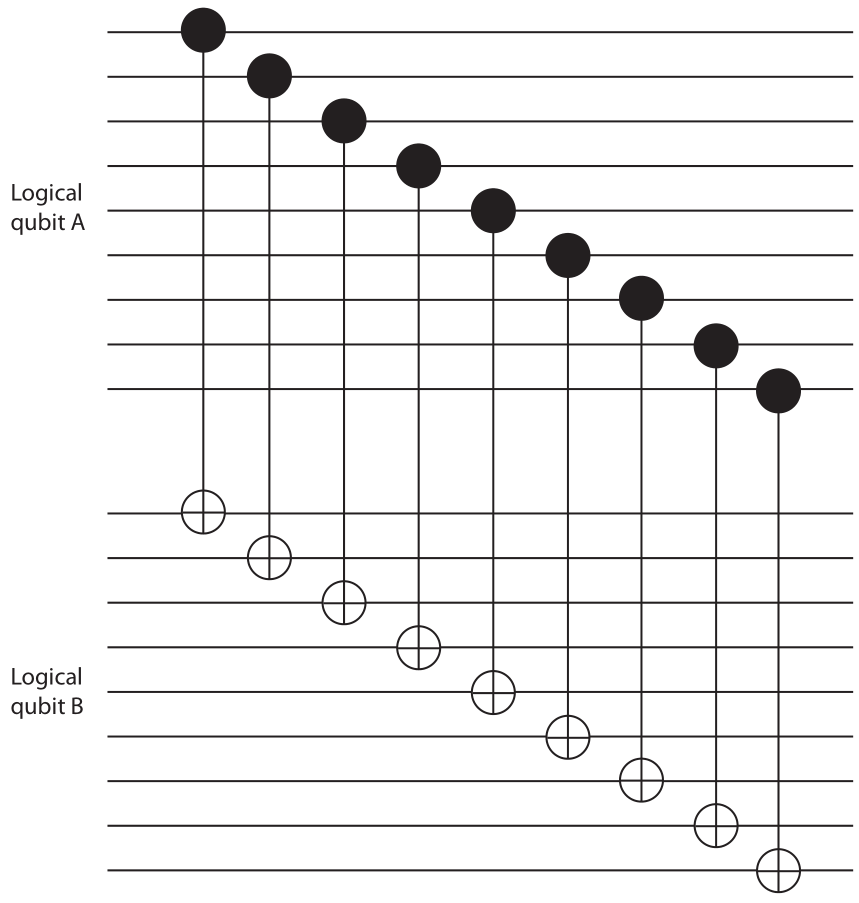
\includegraphics[width=.4\textwidth]{problem-4.png}\end{center}

    What operation does this circuit perform on the two logical qubits? (Hint: It's not quite what you think of at first glance!).

    \begin{answer}
        There are four cases to be considered because both $A$ and $B$ can be in either $\ket{0_{Shor}}$ or $\ket{1_{Shor}}$.

        The Shor states consist of three parts as seen in previous exercises and we will look at them one at a time.

        The set is in the state $\rsqrt{2}\left(\ket{000} \pm \ket{111}\right)$. Since we do a \CNOT{} on single qubits from $A$ and $B$ we can look at the problem from the perspective of qubits $q_{A,n}$ and $q_{B,n}$. But, I want to write them shorter so these qubits are now $a$ and $b$ respectively.

        Using the following definitions:
        \begin{align*}
            \ket{+} = \rsqrt{2}\left(\ket{0} + \ket{1}\right) \\
            \ket{-} = \rsqrt{2}\left(\ket{0} - \ket{1}\right)
        \end{align*}
        We can calculate the result of applying \CNOT{ab} to the 4 possible combinations of the states of $a$ and $b$:
        \begin{align*}
            a \otimes b ~~~& ~~~~~~~\CNOT{ab} \\
            \ket{+} \otimes \ket{+} & \rightarrow \ket{+} \otimes \ket{+} \\
            \ket{+} \otimes \ket{-} & \rightarrow \ket{-} \otimes \ket{-} \\
            \ket{-} \otimes \ket{+} & \rightarrow \ket{-} \otimes \ket{+} \\
            \ket{-} \otimes \ket{-} & \rightarrow \ket{+} \otimes \ket{-}
        \end{align*}
        The strange thing is that $a$ actually gets phase flipped if $b = \ket{-}$.
        Now we can extend this to the level of logical qubits and we get that:
        \begin{align*}
            \ket{0_{Shor}} \otimes \ket{0_{Shor}} &\rightarrow \ket{0_{Shor}} \otimes \ket{0_{Shor}} \\
            \ket{0_{Shor}} \otimes \ket{1_{Shor}} &\rightarrow \ket{1_{Shor}} \otimes \ket{1_{Shor}} \\
            \ket{1_{Shor}} \otimes \ket{0_{Shor}} &\rightarrow \ket{1_{Shor}} \otimes \ket{0_{Shor}} \\
            \ket{1_{Shor}} \otimes \ket{1_{Shor}} &\rightarrow \ket{0_{Shor}} \otimes \ket{1_{Shor}}
        \end{align*}
        So, the \CNOT{ab}'s actually implement a logical \CNOT{BA}.
    \end{answer}
\end{enumerate}

These were mostly fun and valuable exercises :), thank you for your effors so far I really appreciate it!

Happy holidays!

\begin{center}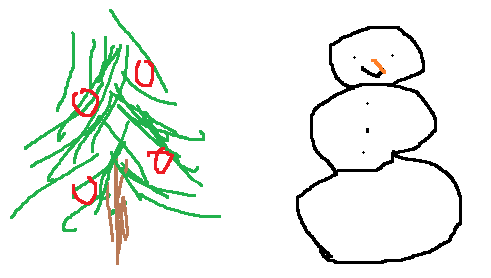
\includegraphics[width=.4\textwidth]{happy-holidays.png}\end{center}
\end{document}

